% ----------------------------------
% 1-Preambulo.
% ----------------------------------
\documentclass[12pt,a4paper]{article}
\usepackage[spanish]{babel}
\usepackage[T1]{fontenc}
\usepackage{textcomp}
\usepackage{lmodern}
\usepackage[utf8]{inputenc}
\usepackage{graphicx}
\usepackage[procnames]{listings} 	%Para escribir códigos.
% OJO: se agregaron procnames para usarlos en Python (VER).

\usepackage[bottom]{footmisc} 	 	%Para poner las footnote al final de cada página.
\usepackage[hidelinks]{hyperref} 	%Para que el indice pueda ser linkeado.
\usepackage{amssymb}			 	%Para ecuaciones matemáticas.
\usepackage{amsmath}				%Para matrices.
\usepackage{mathtools}
\usepackage{amsfonts} 
\usepackage{verbatim}				%Para usar comentarios.
\parskip 0.1in 						%Distancia parrafos.

%Biliografías:
%\usepackage[style=authoryear]{biblatex}
%\addbibresource{bibliografias.bib}

\usepackage{float} 							%Para que no se muevan las imágenes de lugar.

\usepackage[
  separate-uncertainty = true,
  multi-part-units = repeat
]{siunitx} 									%Para el \SI del +- .

\usepackage[margin=0.984252in]{geometry} 	%Para los márgenes.
\usepackage{subcaption}
\usepackage{appendix} 						%Para los anexos.

% ----------------------------------
% 1.1-Anexos.
% ----------------------------------

%begin anexos
\makeatletter
\def\@seccntformat#1{\@ifundefined{#1@cntformat}  	%"\@seccntformat" es un comando auxiliar.
   {\csname the#1\endcsname\quad}  					%Default.
   {\csname #1@cntformat\endcsname}					%Enable individual control.
}

\let\oldappendix\appendix 							%Guarda la definicion vigente de \appendix
\renewcommand\appendix{%
    \oldappendix
    \newcommand{\section@cntformat}{\appendixname~\thesection\quad}
}
\makeatother
%\renewcommand{\appendixname}{Anexos}
%\renewcommand{\appendixtocname}{Anexos}
%\renewcommand{\appendixpagename}{Anexos}
%end anexos

% ----------------------------------
% 1.2-Para código Python. 
% ----------------------------------
\usepackage{color}
\definecolor{keywords}{RGB}{255,0,90}
\definecolor{comments}{RGB}{0,0,113}
\definecolor{red}{RGB}{160,0,0}
\definecolor{green}{RGB}{0,150,0}
 
\lstset{language=Python, 
        basicstyle=\ttfamily\small, 
        keywordstyle=\color{keywords},
        commentstyle=\color{comments},
        stringstyle=\color{red},
        showstringspaces=false,
        identifierstyle=\color{green},
        procnamekeys={def,class}}

% ----------------------------------
% 1.3-Índice. 
% ----------------------------------

\setcounter{secnumdepth}{3} 		%Para que ponga 1.1.1.1.
\setcounter{tocdepth}{4} 			%Para que añadir las secciones en el Índice.
\usepackage{chngcntr}				%Para que el número de las figuras esten acordes a la sección.
\counterwithin{figure}{section}

\author{
  Calonge, Federico Matias\\
  \text{calongefederico@gmail.com}
}

\title{
  Tesis \\
  \large Automatización de lectura de Currículum Vitae  \\
    para selección de personal en el Sector IT}
    
%Para modificar los parrafos y para que se pueda poner subsections:
\makeatletter
\renewcommand\paragraph{\@startsection{paragraph}{4}{\z@}
            {-2.5ex\@plus -1ex \@minus -.25ex}
            {1.25ex \@plus .25ex}
            {\normalfont\normalsize\bfseries}}
\makeatother
\setcounter{secnumdepth}{4} 	%How many sectioning levels to assign numbers to.
\setcounter{tocdepth}{4}    	%How many sectioning levels to show in ToC.
% ----------------------------------
% 2-Documento
% ----------------------------------

\begin{document}

\begin{figure}
  \centering
  
\includegraphics[width=0.2\textwidth]{images/undav-logo.png} 	%Incluyendo logo de la Undav.
  \label{fig:undav-logo}
\end{figure}
\maketitle       		%Para generar el título definido arriba.

\cleardoublepage    %Nueva página

\begin{center}
    \Large
    \vspace{0.9cm}
    \textbf{Resumen}
    
\end{center}

En la Tesis de Ingeniería que se presenta, se diseña un \textit{sistema de lectura automática de Curriculum Vitae}. La finalidad del mismo es ayudar al reclutador laboral a elegir a los mejores candidatos para los puestos laborales que tenga disponible mediante una medición de similitud entre textos: Curriculum Vitae de los candidatos por un lado, y descripciones de puestos laborales por el otro.
El sistema esta desarrollado utilizando el lenguaje de programación Python, permitiendo verificar la teoría desarrollada.

\begin{center}
    \Large
    \vspace{0.9cm}
    \textbf{Abstract}
\end{center}

This Engineering Thesis introduces an \textit{automatic Curriculum Vitae reading system}. The purpose of it is to help the job recruiter to choose the best candidates for the available job positions by means of a measurement of similarity between texts: Curriculum Vitae of the candidates on the one hand, and job descriptions on the other. The system is developed using the Python programming language allowing to verify the developed theory.

\cleardoublepage    %Nueva página

\tableofcontents 	%Para insertar el índice general.

\cleardoublepage    %Nueva página

\section{Introducción.}
El proceso de \textbf{selección de personal} se ha vuelto crucial para el manejo de recursos humanos en el mundo laboral moderno. Con la transformación digital de las empresas y del mercado laboral en general, identificar los perfiles más acordes a las necesidades de la empresa se convirtió en uno de los retos más ambiciosos de Recursos Humanos, en especial cuando hablamos del \textbf{Sector IT}. 

En estos últimos años se implementaron una gran cantidad de \textbf{herramientas de Software que permiten automatizar y gestionar información de los candidatos de una manera mucho más intuitiva e inteligente}. Gracias a la ayuda de este tipo de sistemas, el reclutador consigue a los candidatos más cualificados para cada puesto.

El tema de este Proyecto de Tesis será desarrollar un \textbf{Sistema de lectura automática de Curriculum Vitae} que ayude al reclutador laboral a elegir a los mejores candidatos para los puestos laborales que tenga disponible mediante una \textbf{medición de similitud} entre textos: los Curriculum Vitae de los candidatos por un lado, y las descripciones de puestos laborales por el otro.

La medición de similitudes de documentos es uno de los problemas más cruciales del \textbf{Procesamiento del Lenguaje Natural (NLP)}. Encontrar similitudes entre documentos se utiliza en varios dominios, tales como recomendación de películas, libros o artículos similares, identificación de documentos plagiados o documentos legales, etc. 

Para que las máquinas puedan descubrir esta similitud entre documentos, se necesita definir una forma de medir matemáticamente la similitud, la cual debe ser comparable para que la máquina pueda identificar qué documentos son más similares (o menos). Previamente a esto necesitamos representar el texto de los documentos en una forma cuantificable (que suele ser en forma vectorial), de modo que podamos realizar cálculos de similitud sobre él.

Por lo tanto, los pasos necesarios para que las máquinas puedan medir la similitud entre documentos son:
\begin{enumerate}
\item Convertir un documento en un objeto matemático (vector).
\item Definir y emplear una medida de similitud.
\end{enumerate}

Para el primer paso se utilizarán los algoritmos de vectorización \textbf{TF-IDF} y \textbf{Word Embeddings}; y para el segundo paso se emplearán las técnicas \textbf{Cosine Similarity} y \textbf{Word Mover's Distance -WMD-}.

\cleardoublepage    %Nueva página

\subsection{Objetivos del Proyecto.}

\subsubsection{Objetivo general.}
El objetivo de este Proyecto de Tesis es lograr la implementación de un Sistema de lectura automática de Curriculum Vitae accesible vía Web, que servirá para la elección de los mejores candidatos para cada puesto laboral; basándose en la \textbf{similitud} entre el Currículum Vitae del candidato y el puesto laboral. 

\subsubsection{Objetivos específicos.}
Los objetivos específicos de este Proyecto de Tesis son:
\begin{itemize}
\item Describir el estado del arte actual de los Sistemas de lectura y análisis de Curriculum Vitae en Recruiting. 
\item Implementar un Sistema de lectura automática de Curriculum Vitae basado en la comparación entre textos, para finalmente obtener una visualización de los mejores candidatos para un puesto laboral determinado.  
\item Aprender los conceptos y técnicas principales utilizadas dentro del procesamiento de lenguaje natural (NLP) aplicando técnicas de preprocesamiento y limpieza de textos.
\item Implementar diferentes técnicas para medir similitudes entre los textos (Cosine Similarity y  Word Mover's Distance -WMD-) y diferentes algoritmos de vectorización (TF-IDF y Word Embeddings), analizando su funcionamiento tanto teórica como matemáticamente, ventajas y desventajas.
\item Evaluar los resultados de cada técnica y algoritmo e implementar la mejor solución en el Sistema.
\item Evaluar los Frameworks disponibles para tener una UI accesible vía web e integrar el mismo al Sistema.
\item Almacenar datos de Candidatos, Reclutadores y puestos laborales en una base de datos; contando con un sistema de login y registración para los mismos.
\end{itemize} 


\cleardoublepage    %Nueva página

\subsection{Alcance del Proyecto.}
El alcance de esta Tesis de Grado de Ingeniería incluye el desarrollo de conceptos de análisis de datos, procesamiento de lenguaje natural, técnicas de preprocesamiento y limpieza de los datos, algoritmos de vectorización y técnicas para medir la similitud entre textos, integración con frameworks, visualización de datos, y gestión de Base de Datos, de acuerdo a lo enunciado en los objetivos específicos.

\subsection{Organización.}
Texto ejemplo. Texto ejemplo. Texto ejemplo. Texto ejemplo. Texto ejemplo. Texto ejemplo.

\section{Reclutamiento laboral en IT.}
Texto ejemplo. Texto ejemplo. Texto ejemplo. Texto ejemplo. Texto ejemplo. Texto ejemplo.

\subsection{Introducción.}
Texto ejemplo. Texto ejemplo. Texto ejemplo. Texto ejemplo. Texto ejemplo. Texto ejemplo.

\subsection{Problemáticas.}
Texto ejemplo. Texto ejemplo. Texto ejemplo. Texto ejemplo. Texto ejemplo. Texto ejemplo.

\subsection{Sistemas de lectura y análisis de CV : Estado del arte.}
Texto ejemplo. Texto ejemplo. Texto ejemplo. Texto ejemplo. Texto ejemplo. Texto ejemplo.

\section{Aprendizaje supervisado y no supervisado en Machine Learning.}

\subsection{Introducción.}
Texto ejemplo. Texto ejemplo. Texto ejemplo. Texto ejemplo. Texto ejemplo. Texto ejemplo.
Los métodos que utilizaremos en este Proyecto de Tesis serán...

\subsection{K-Nearest Neighbor (KNN).}
K-Nearest Neighbor (o K Vecinos más Próximos en español), blablabal....

\subsection{K-Means.}
K-Means (o K-Medias en español), blablaba...

\subsubsection{Elbow Method.}
Elbow Method (o Método del codo en español), blablaba...

\section{Natural Language Processing.}
Texto ejemplo. Texto ejemplo. Texto ejemplo. Texto ejemplo. Texto ejemplo. Texto ejemplo.

\subsection{Introducción.}
Texto ejemplo. Texto ejemplo. Texto ejemplo. Texto ejemplo. Texto ejemplo. Texto ejemplo.

\subsection{Preprocesamiento de textos.}
Texto ejemplo. Texto ejemplo. Texto ejemplo. Texto ejemplo. Texto ejemplo. Texto ejemplo.

\subsection{Similitud entre textos.}
Texto ejemplo. Texto ejemplo. Texto ejemplo. Texto ejemplo. Texto ejemplo. Texto ejemplo.

\subsection{Técnicas para medir Similitud entre textos.}
Texto ejemplo. Texto ejemplo. Texto ejemplo. Texto ejemplo. Texto ejemplo. Texto ejemplo.

\subsubsection{Cosine Similarity.}
Texto ejemplo. Texto ejemplo. Texto ejemplo. Texto ejemplo. Texto ejemplo. Texto ejemplo.

\subsubsection{Word Mover's Distance (WMD).}
Texto ejemplo. Texto ejemplo. Texto ejemplo. Texto ejemplo. Texto ejemplo. Texto ejemplo.

\subsection{Algoritmos de vectorización.}
Texto ejemplo. Texto ejemplo. Texto ejemplo. Texto ejemplo. Texto ejemplo. Texto ejemplo.

\subsubsection{TF-IDF.}
Texto ejemplo. Texto ejemplo. Texto ejemplo. Texto ejemplo. Texto ejemplo. Texto ejemplo.

\subsubsection{Word Embeddings.}
Texto ejemplo. Texto ejemplo. Texto ejemplo. Texto ejemplo. Texto ejemplo. Texto ejemplo.

\paragraph{¿Cómo entrenar Word Embeddings?}
Texto ejemplo. Texto ejemplo. Texto ejemplo. Texto ejemplo. Texto ejemplo. Texto ejemplo.

\section{Desarrollo.}
Texto ejemplo. Texto ejemplo. Texto ejemplo. Texto ejemplo. Texto ejemplo. Texto ejemplo.

\subsection{Introducción.}
El desarrollo de este Sistema se realizó en Python...

\subsection{Esquema del sistema.}
Como podemos ver en la figura \ref{fig:FlowCoreSystem}, blablaba. \\

\begin{figure}[h]    %[h] es para que se ubique justo debajo del texto anterior. 
  \centering
  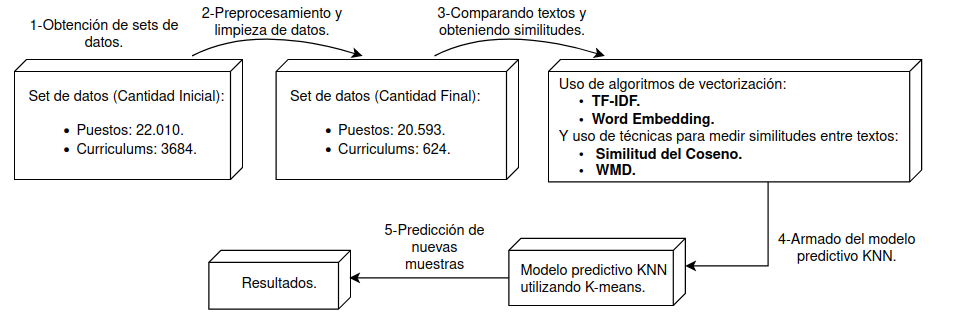
\includegraphics[width=1\textwidth]{images/flow-core.png} 	%Incluyendo imagen Flow Core.
  \caption{Flow del Core del Sistema}  
  \label{fig:FlowCoreSystem}
\end{figure}

\subsection{Set de datos.}
Un Set o conjunto de datos es una tabla de una base de datos o, matemáticamente, una matriz estadística de datos. Cada columna de la tabla representa una variable del Data Set; y cada fila representa a un miembro determinado del conjunto de datos.

Previamente a utilizar algoritmos de ......
necesitamos que los datos estén limpios, por esta razón es importantísimo manipular y analizar estos
datos en una primera instancia para luego si, meter estos datos limpios en los algoritmos y que estos
funcionen correctamente; ya que de lo contrario las máquinas podrían clasificar o predecir de forma
errónea. Este análisis previo sobre los datos debe ser minucioso ya que puede haber valores
incoherentes o absurdos.

Para este Proyecto utilizamos dos grandes sets de datos, descriptos a continuación.

\subsubsection{Curriculum Vitae.}
Texto ejemplo. Texto ejemplo. Texto ejemplo. Texto ejemplo. Texto ejemplo. Texto ejemplo.

\subsubsection{Descripciones Puestos Laborales.}
Texto ejemplo. Texto ejemplo. Texto ejemplo. Texto ejemplo. Texto ejemplo. Texto ejemplo.

\subsection{Medición de similitud entre textos.}
Texto ejemplo. Texto ejemplo. Texto ejemplo. Texto ejemplo. Texto ejemplo. Texto ejemplo.

\subsubsection{FALTA: Pasos de las pruebas que hice: "Mejorando…" / "Implementación de…" / "Problemas al…".}
Texto ejemplo. Texto ejemplo. Texto ejemplo. Texto ejemplo. Texto ejemplo. Texto ejemplo.

\subsection{Resultados Obtenidos.}
Texto ejemplo. Texto ejemplo. Texto ejemplo. Texto ejemplo. Texto ejemplo. Texto ejemplo.

\subsection{Conclusiones.}
Texto ejemplo. Texto ejemplo. Texto ejemplo. Texto ejemplo. Texto ejemplo. Texto ejemplo.

\subsection{Agregando funcionalidades.}
Texto ejemplo. Texto ejemplo. Texto ejemplo. Texto ejemplo. Texto ejemplo. Texto ejemplo.

\subsubsection{Base de datos.}
Texto ejemplo. Texto ejemplo. Texto ejemplo. Texto ejemplo. Texto ejemplo. Texto ejemplo.

\subsubsection{Framework Web.}
Texto ejemplo. Texto ejemplo. Texto ejemplo. Texto ejemplo. Texto ejemplo. Texto ejemplo.

\subsubsection{Roles y Usuarios.}
Texto ejemplo. Texto ejemplo. Texto ejemplo. Texto ejemplo. Texto ejemplo. Texto ejemplo.

\subsubsection{Manejo de los datos.}
Texto ejemplo. Texto ejemplo. Texto ejemplo. Texto ejemplo. Texto ejemplo. Texto ejemplo.

\paragraph{Modelado.}
Texto ejemplo. Texto ejemplo. Texto ejemplo. Texto ejemplo. Texto ejemplo. Texto ejemplo.

\paragraph{Filtrado.}
Texto ejemplo. Texto ejemplo. Texto ejemplo. Texto ejemplo. Texto ejemplo. Texto ejemplo.

\paragraph{Visualización.}
Texto ejemplo. Texto ejemplo. Texto ejemplo. Texto ejemplo. Texto ejemplo. Texto ejemplo.

\subsection{Caso de Uso.}
Texto ejemplo. Texto ejemplo. Texto ejemplo. Texto ejemplo. Texto ejemplo. Texto ejemplo.

\subsection{Limitaciones del sistema.}
Texto ejemplo. Texto ejemplo. Texto ejemplo. Texto ejemplo. Texto ejemplo. Texto ejemplo.
 
\section{Próximos pasos.}  
Texto ejemplo. Texto ejemplo. Texto ejemplo. Texto ejemplo. Texto ejemplo. Texto ejemplo.

\section{Glosario.}
Texto ejemplo. Texto ejemplo. Texto ejemplo. Texto ejemplo. Texto ejemplo. Texto ejemplo.

\section{Anexo.}
Texto ejemplo. Texto ejemplo. Texto ejemplo. Texto ejemplo. Texto ejemplo. Texto ejemplo.

\section{Bibliografía.}
Texto ejemplo. Texto ejemplo. Texto ejemplo. Texto ejemplo. Texto ejemplo. Texto ejemplo.

\section{Agradecimientos.}
Texto ejemplo. Texto ejemplo. Texto ejemplo. Texto ejemplo. Texto ejemplo. Texto ejemplo.

\end{document}


%Para poner pie de paginas --> \footnote{Un conjunto de datos, conocido también como dataset, es una colección de datos habitualmente tabulada.})

%Para poner en Las citas del anexo --> información\cite{iot}. 

